\documentclass[11pt]{jarticle}

\usepackage[dvipdfmx]{graphicx}

\setlength{\oddsidemargin}{-6.35mm}
\setlength{\textwidth}{171.9mm}

\begin{document}

\title{画像処理実験 第7回}
\author{09430509\\今田将也}
\date{\number\year 年\number\month 月\number\day 日}
\maketitle

\section{RANSAC(あるいは独自の方法)で自動対応付けを実現し,画像を合成しなさい}

パノラマ画像での各画像から抽出してきた特徴量は,もう一方の画像に対応点が存在していない「外れ値」が含まれており,
最小二乗法によりどの点とどの点が対応するかを計算すると,外れ値ではうまく対応関係が作れない.
そこで、パノラマ画像作成での対応点計算にはRANSACにより外れ値は見ないような上手い対応点を見つける.

RANSACでは以下の3つの手続きを最適な評価値(スコア)が(3)で出てくるまで繰り返す
(1):あらかじめ決めておいたサンプル数nだけランダムにデータをサンプリング
(2):サンプルしたn個のデータを用い,モデルのパラメータを算出(最小二乗法で誤差を最小化)
(3):処理2で求めたモデルのパラメータに対して、あらかじめ範囲を決めておいた閾値内のデータのみを用いて,どれくらい正しいかのスコアを評価

この(1)~(3)の処理による各繰り返しにおいて,外れ値ではない正しい特徴点ができているかを判断する.

\subsection{問題点}
試行回数が少ないと上手く合成できない.閾値が適正でないと上手く合成できない.

\subsection{改善策}
試行回数を増やし,閾値を小さくすることで改善できた.
試行回数は対応点集合の中に含まれる誤りの割合を p とすることで見積もることができるが今回は余力がないためやっていない.

\section{下記の観点で考察または実装しなさい}
\subsection{4つの乱数(i0,i1,i2,i3)を発生させるとき,同じものが2度以上選ばれないようにする方法}
以下実装したソースコードである.
\begin{verbatim}
    void initRndAry(int rndAry[MAX]){
        for(int i = 0; i<MAX; i++){
            rndAry[i] = i;
        }
        srand(__rdtsc()); // __rdtsc については第4回を参照
    }

    void chooseFourNumbers(int rndAry[MAX]){
        for(int i=0;i<4;i++){
            int j, t;
            j = (int)((long long)rand()*(MAX-i)/(RAND_MAX+1LL))+i; // 乱数関数は stdlib.h で宣言されている.
            t = rndAry[i]; 
            rndAry[i] = rndAry[j]; 
            rndAry[j] = t;
        }
    }
\end{verbatim}
rndAry は,0 から MAX-1 までの数を 1 つずつ保持している. この配列の内容を入れ替える操作によって,数値の順序は変わるが,
全ての数値が一回づつ現れる性質は変わらないため, 相異なる数個の乱数が得られる.

上記の rndAry[0] から rndAry[3] を使う部分では,配列 w[][4] から4行を選んで変換行列を算出する
以下にそのソースコードを示した.

\begin{verbatim}
    void calcHomography(double H[3][3],double w[][4],int rndAry[MAX], Matrix *cmA, Matrix *vt, Matrix *mtR, Matrix *tmp){
    int a = rndAry[0], b = rndAry[1], c = rndAry[2], d = rndAry[3];
    double ww[][4] = {
        w[a][0], w[a][1], w[a][2], w[a][3],
        w[b][0], w[b][1], w[b][2], w[b][3],
        w[c][0], w[c][1], w[c][2], w[c][3],
        w[d][0], w[d][1], w[d][2], w[d][3],
    };
      // create A (col-major)
    for(int i=0;i<4;i++){
        Elem(cmA,0,i*2  )=ww[i][0];
        Elem(cmA,1,i*2  )=ww[i][1];
        Elem(cmA,2,i*2  )=1;
        Elem(cmA,3,i*2  )=0;
        Elem(cmA,4,i*2  )=0;
        Elem(cmA,5,i*2  )=0;
        Elem(cmA,6,i*2  )=-ww[i][0]*ww[i][2];
        Elem(cmA,7,i*2  )=-ww[i][1]*ww[i][2];
        Elem(cmA,0,i*2+1)=0;
        Elem(cmA,1,i*2+1)=0;
        Elem(cmA,2,i*2+1)=0;
        Elem(cmA,3,i*2+1)=ww[i][0];
        Elem(cmA,4,i*2+1)=ww[i][1];
        Elem(cmA,5,i*2+1)=1;
        Elem(cmA,6,i*2+1)=-ww[i][0]*ww[i][3];
        Elem(cmA,7,i*2+1)=-ww[i][1]*ww[i][3];
        Elem(vt ,0,i*2  )=ww[i][2];
        Elem(vt ,0,i*2+1)=ww[i][3];
    }
    MatrixQRDecompColMajor(mtR,cmA);
    MatrixMultT(tmp,vt,cmA);
    MatrixSimeqLr(tmp,mtR);

    H[0][0] = Elem(tmp,0,0);
    H[0][1] = Elem(tmp,0,1);
    H[0][2] = Elem(tmp,0,2);
    H[1][0] = Elem(tmp,0,3);
    H[1][1] = Elem(tmp,0,4);
    H[1][2] = Elem(tmp,0,5);
    H[2][0] = Elem(tmp,0,6);
    H[2][1] = Elem(tmp,0,7);
    H[2][2] = 1;
}
\end{verbatim}

そして,変換行列の信頼度を評価するため,上記の「検出された点と変換された点の距離が十分に小さい点」の数を計算する.
以下そのソースコード部分である.
\begin{verbatim}
    int calcScore(double H[3][3], double w[][4]){
        int score=0;
        for(int i=0;i<MAX;i++){
            double x=w[i][0], y=w[i][1], u=w[i][2], v=w[i][3],
            x_prime = H[0][0] * x + H[0][1] * y + H[0][2],
            y_prime = H[1][0] * x + H[1][1] * y + H[1][2],
            z_prime = H[2][0] * x + H[2][1] * y + H[2][2], // 変換行列と (x,y,1)^T の積
            du = (x_prime/z_prime) - u,
            dv = (y_prime/z_prime) -v; // (x,y) を変換した座標(第2回の概要を参照)と (u,v) の差
            if(du*du+dv*dv < 10) score++;//w[i] は正しい;
            else score += 0;              //w[i] は正しくない;
        }
        return score;
    }    
\end{verbatim}

この実装により得られた画像は図\ref{last}に示した.

\begin{figure}[ht]
\centering
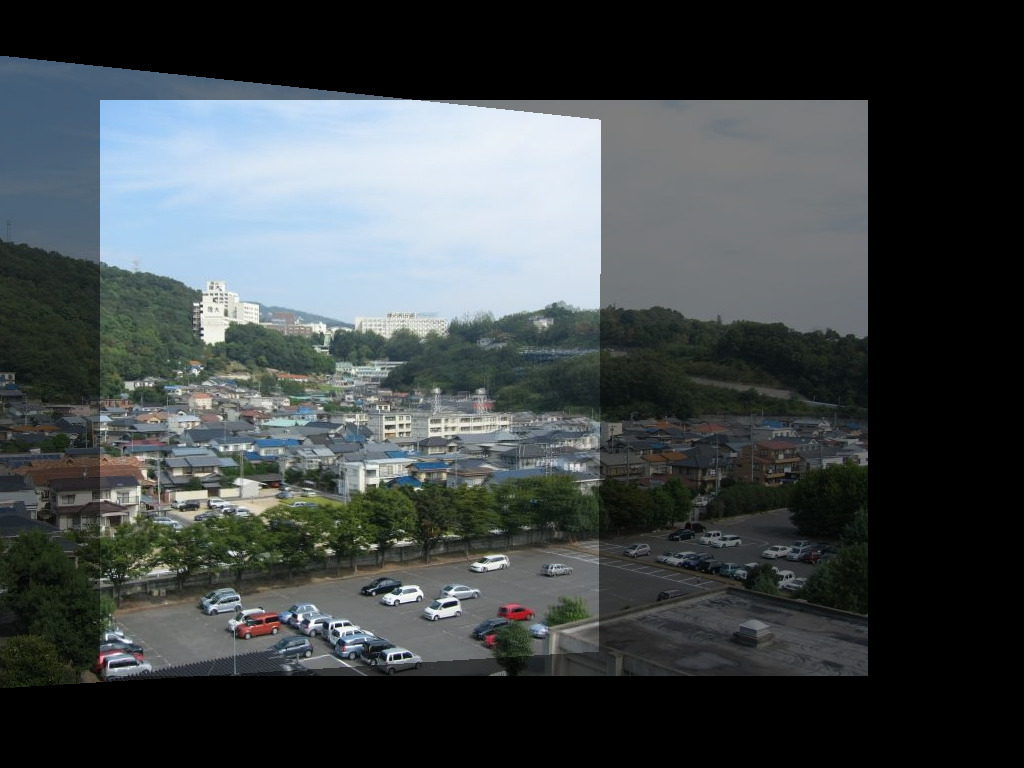
\includegraphics[scale=.5]{dai8.jpg}
\caption{結果}
\label{last}
\end{figure}

\section{感想}
今まで作ってきたものを上手く組み合わせたり,ヘッダーファイルやimage.cに書き込むことで
実装をすすめることができた.ただ,深く実装を理解していたわけではなかったので,移し替えるときに
どこをどうやって書き換えればいいのか悩み時間を溶かしたがなんとかできた.

来週の最終レポートではここまでの内容をまとめ,復習をしておきたい.

\end{document}
